% !TEX root = ../main.tex

\clearpage

\section{Protocol Diagram}

\begin{figure}[ht!]
    %---------------------------------------left, bottom, right, top
    \vspace{-1cm}
    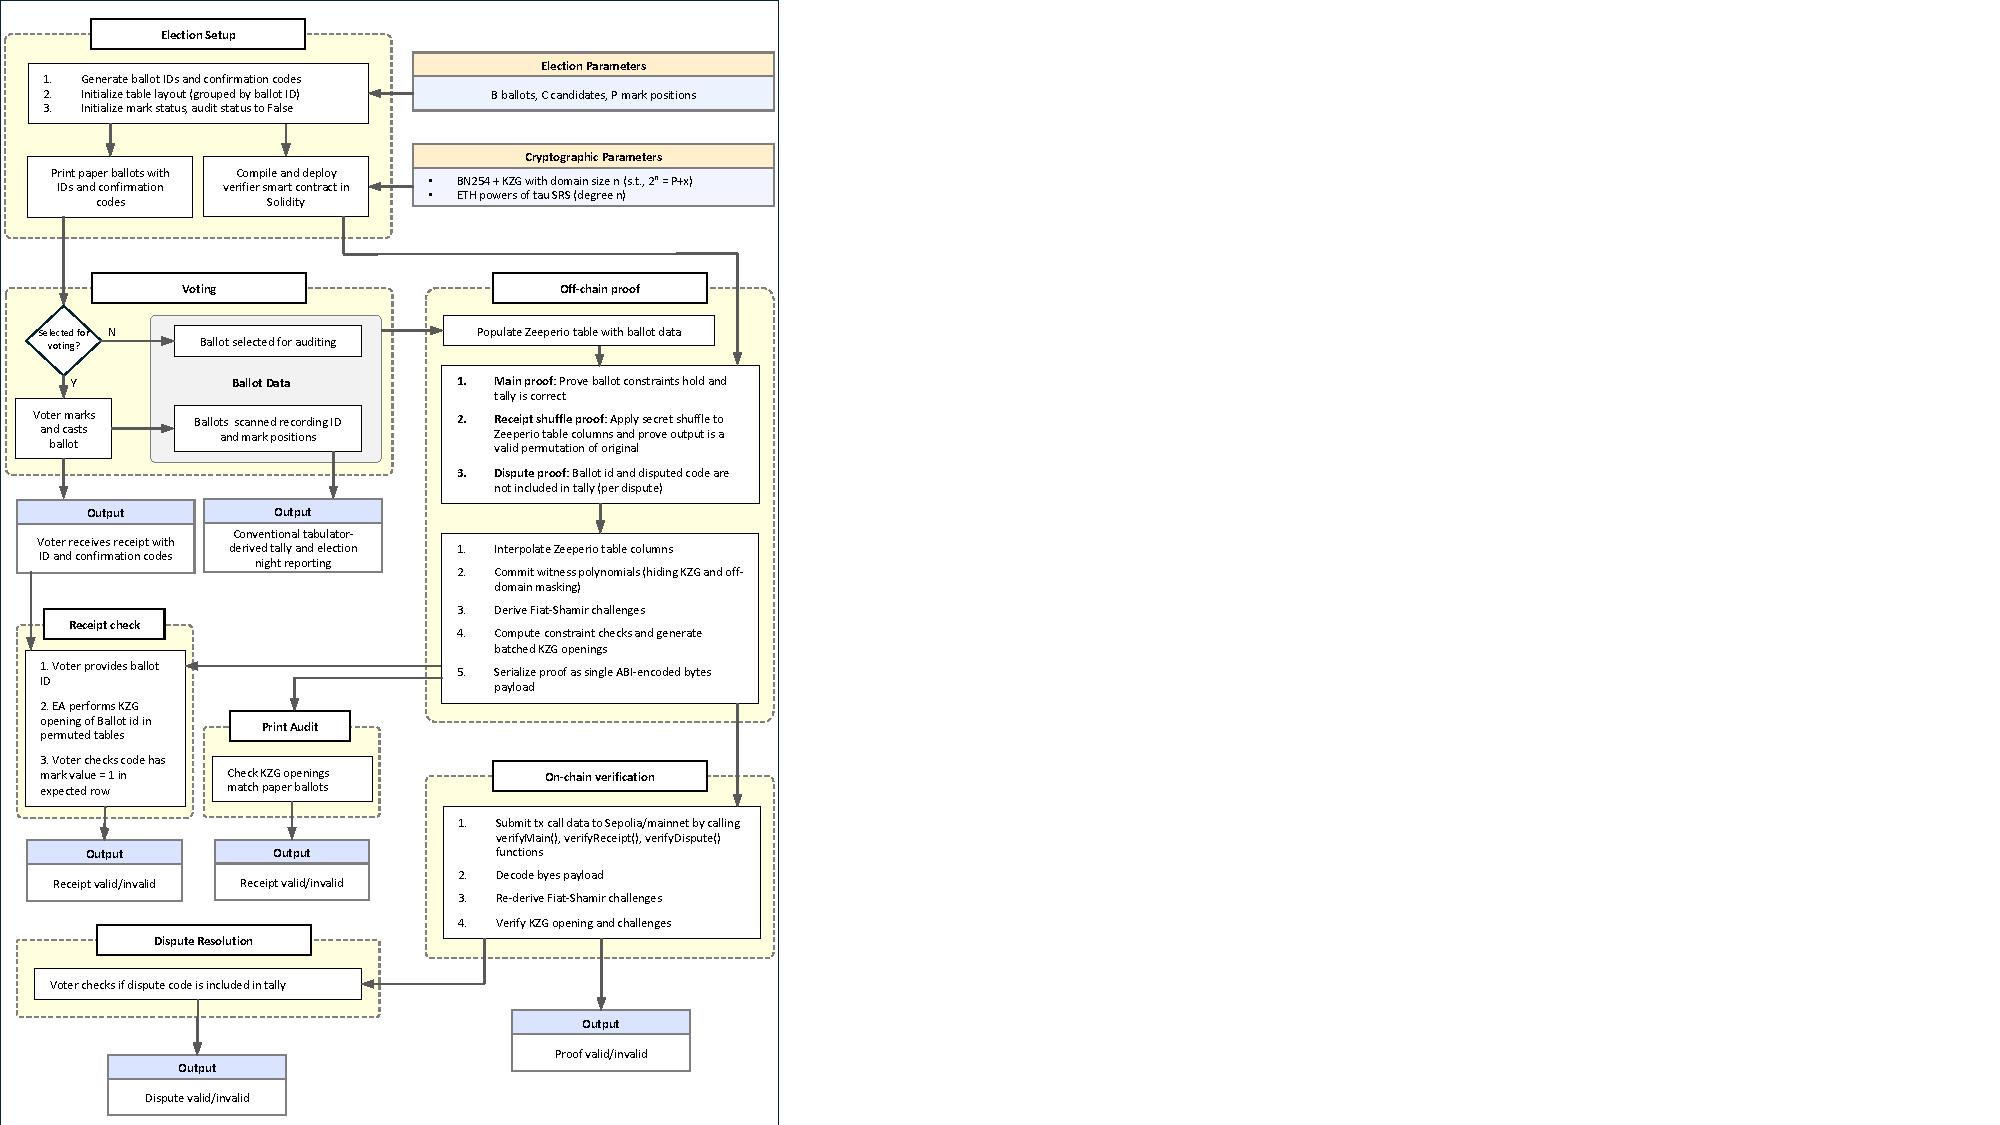
\includegraphics[width=\linewidth, trim={0.02cm, 0cm, 20.7cm, 0.04cm}, clip]{figures/protocol.pdf}
    \caption{Protocol Diagram.}
    \label{fig:protocol-diagram}
\end{figure}

\clearpage

\section{A}
As shown in Fig. \ref{fig:zklevel}, there are several ways of building a SNARK system. SNARKs are typically implemented at a higher abstraction level with a \emph{circuit}, or a \emph{program} running inside a zkVM.
The program is first converted into a circuit representation. The circuit is then compiled into a constraint system represented by Poly-IOP gadgets. 
These gadgets consist of selector polynomials, wire polynomials, permutation arguments, and grand-product checks \cite{Liang:2025:SoK}.

\begin{figure}[H]
\centering
\resizebox{\textwidth}{!}{
\begin{tikzpicture}[
    >=Stealth,
    node distance=3.0cm,
    box/.style={draw, rounded corners=4pt,
                minimum width=3.10cm, minimum height=1.10cm,
                align=center},
    lab/.style={font=\scriptsize},
    small/.style={font=\scriptsize, align=center},
    every node/.style={font=\footnotesize}
]

\node[box]                       (zkvm)  {zkVM\\\scriptsize(assembly)};
\node[box, right=of zkvm]        (circ)  {Circuit / zkDSL\\\scriptsize(gates/constraints)};
\node[box, right=of circ]        (gadg)  {Poly-IOP Gadgets\\\scriptsize(polynomial identities)};
\node[box, right=3.4cm of gadg]  (zkp)   {Proof};

\draw[->] (zkvm.east) -- (circ.west);
\draw[->] (circ.east) -- (gadg.west);
\draw[->] (gadg.east) -- (zkp.west);

\node[box, above=1.9cm of circ] (snark) {SNARK\\\scriptsize(compiler \& argument)};
\draw[->, dashed] (snark.south west) to[bend right=18] (zkvm.north);
\draw[->, dashed] (snark.south)      to[bend right=10] (circ.north);
\draw[->, dashed] (snark.south east) to[bend left=10]  (gadg.north);

\node[lab, above=0.30cm of zkvm] {Layer 1: VM-level};
\node[lab, above=0.30cm of circ] {Layer 2: Circuit-level};
\node[lab, above=0.30cm of gadg] {Layer 3: Polynomial-level};

\node[small, below=0.55cm of zkvm]  {highest overhead\\largest constraints\\heaviest prover cost};
\node[small, below=0.55cm of circ]  {moderate overhead\\generic circuits\\compiler-friendly};
\node[small, below=0.55cm of gadg]  {closest to the metal\\domain-specific structure\\lowest overhead};

\draw[very thick, ->]
  ([yshift=-2.05cm] zkvm.south west) --
  node[lab, below, pos=0] {least efficient / most overhead}
  node[lab, below, pos=1] {most efficient / least overhead}
  ([yshift=-2.05cm] gadg.south east);

\node[lab, above]
  at ($(zkvm.south)!0.5!(gadg.south) + (0,-2.6cm)$)
  {moving right $\Rightarrow$ \emph{closer to the metal}};

\end{tikzpicture}%
}
\caption{Three layers of abstraction for constructing succinct proofs. From left to right, the prover’s statement is expressed at (i) the VM level (zkVM), (ii) the circuit level, or (iii) directly as Poly-IOP gadgets (polynomial identities). Shifting right is “closer to the metal” as it goes directly to the cryptography level. 
This reduces constraint and compilation overhead resulting in more efficient proofs, leading to cheaper verification.}
\label{fig:zklevel}
\end{figure}


\section{Setup Phase}
\label{subsec:setup-phase}

Like many Poly-IOP-based systems, Zeeperio begins with a trusted setup phase to generate a Structured Reference String (SRS). We use Ethereum's \textit{Powers of Tau} ceremony, a public multi-party computation that produces a universal and updatable SRS composed of elliptic curve group elements
\[
\text{SRS} = \left(g, g^\tau, g^{\tau^2}, \dots, g^{\tau^d}\right),
\]
where $\tau$ is a secret value discarded after the setup \cite{cryptoeprint:2025/064}. This SRS supports pairing-based cryptography and is used to commit to polynomials in the KZG scheme.

We use Ethereum's \textit{degree-20} Powers of Tau output, which supports polynomials of degree less than $2^{20} = 1,048,576$. This degree was chosen to comfortably accommodate the maximum expected number of voters at any single polling location. 
With a 20-degree SRS, Zeeperio can support more than one million unique ballot-candidate positions. This ensures there is sufficient capacity even under extreme real-world election conditions.
For example, the Kingston and Islands electoral district has 134,415 residents as of 2025 \cite{ElectionsCanadaDistrictFactSheets2025}. With a 20-degree SRS, Zeeperio can support this district with up to 8 candidates.

The security of the protocol depends on the infeasibility of recovering $\tau$. In this model, no adversary can forge valid proofs without solving discrete logarithms in the elliptic curve group. 
Since we directly use Ethereum's degree-20 Powers of Tau, there is no other trust assumption required and all parameters are public and reusable across all elections.

\section{Audit Column Constraints}
The \textbf{Audit Column} $\mathsf{A}[n]$ is an array of length $n$ that indicates the audit status of ballot $\mathcal{B}_j$.  
For any ballot selected for an audit, $\mathsf{A}[i]=1$ for all its $\mathcal{C}$ positions. In contrast, if the ballot was cast correctly, $\mathsf{A}[i]=0$ for all of its $\mathcal{C}$ positions.

To enforce this, we define a set of constraints that must hold for column $\mathsf{A}$ to be formed correctly:
\begin{itemize}
  \item \textbf{Padding:} The padded values $\mathsf{A}[i]$ where $i \ge \mathcal{P}$ must be 0.
  \item \textbf{Values:} The column $\mathsf{A}$ should contain only 0s or 1s.
  \item \textbf{Blocks:} All $\mathcal{C}$ positions on ballot $\mathcal{B}_j$ must be blocks of 0s or 1s.
  \item \textbf{Count:} The EA publishes $\mathsf{Sum}_A$, the total number of ballots that were audited. We need to enforce the number of 1s in column $\mathsf{A}$ is equal to $\mathsf{Sum}_A \cdot \mathcal{C}$.
\end{itemize}

We now describe how each of these constraints are enforced using Poly-IOP gadgets.

\subsection{Padding}
\label{subsec:padding}
We need to show that $\mathsf{A}[i]=0$ for all padded values $i\ge \mathcal{P}$. This can be achieved by zeroing out all non-padded entries at $0\le i < \mathcal{P}$. As a result, the audit column polynomial $\mathsf{A}(X)$ should evaluate to 0 for every $\omega\in\Omega$.

We define \ref{eq:auditzero}, a constraint specific vanishing polynomial 
with roots at \newline $\{\omega^0, \omega^1, \dots, \omega^{\mathcal{P}-1}\}$:

\begin{equation}
  \label{eq:auditzero}
  \mathsf{Z}(X) = \prod_{i=0}^{\mathcal{P}-1}(X-\omega^i).
\end{equation}

If the audit column padding is implemented correctly, $\mathsf{A}(X)\cdot\mathsf{Z}(X)$ zeros out on the entire evaluation domain $\Omega$. 
For any $i<\mathcal{P}$, $\omega^i$ is a root of $\mathsf{Z}(X)$, 
so $\mathsf{A}(\omega^i)\cdot\mathsf{Z}(\omega^i) = 0$ regardless of $A(\omega^i)$. For $\mathcal{P}\le i<n$ (the padded values), $\mathsf{A}(\omega^i)\cdot\mathsf{Z}(\omega^i) = 0$ iff $\mathsf{A}(\omega^i)=0$. 
Therefore, the domain vanishing polynomial $\mathsf{P_{vanish1}}(X)$ is defined as:


\begin{equation}
  \label{eq:1}
\mathsf{P_{vanish1}}(X) = \mathsf{A}(X)\cdot \mathsf{Z}(X),
\end{equation}
where $\mathsf{P_{vanish1}}(X)=0$ on the evaluation domain $\Omega$.

\subsection{Values}
\label{subsec:values}
We need to show every entry in column $\mathsf{A}[i]$ for $0\le i<n$ is either 0 or 1. The goal is to build a vanishing polynomial $\mathsf{P_{vanish2}}(X)$ such that it zeros out on the entire evaluation domain.
We can achieve this by setting the roots at $\{0,1\}$. Therefore, the domain vanishing polynomial $\mathsf{P_{vanish2}}(X)$ is defined as:
\begin{equation}
  \label{eq:2}
  \mathsf{P_{vanish2}}(X) = \mathsf{A}(X)\cdot (\mathsf{A}(X)-1).
\end{equation}

For any $\mathsf{A}[i]$ set to 1 at indices $0\le i<n$, $\mathsf{A}(X)$ is a root of $\mathsf{P_{vanish2}}(X)$. 
On the other hand, for any $\mathsf{A}[i]$ set to 0, $(\mathsf{A}(X)-1)$ is a also a root of $\mathsf{P_{vanish2}}(X)$.
If $\mathsf{P_{vanish2}}(X)$ zeros out at every $\omega\in\Omega$, the audit column only contains 0s and 1s.

\subsection{Blocks}
\label{subsec:blocks}
For the audit column to be formed correctly, we need to show the audit status for ballot $\mathcal{B}_j$ is consistent among all its $\mathcal{C}$ positions. As shown in Fig. \ref{fig:ballot-columns}, there are three candidates, so the audit column contains the same value for each block of three. 
If we add the values of each block, the result should be either 0 (for the cast ballots), or $\mathcal{C}$ (for the audited ballots).   

We define a block-sum polynomial $\mathsf{S}_{\mathsf{blk}_A}(X)$ where every $X=\omega^i\in\Omega$ corresponds to the sum of the $\mathcal{C}$ consecutive positions in $\mathsf{A}[i]$ for all $0\le i<n$ below:
\begin{equation}
  \label{eq:blksum1}
  \mathsf{S}_{\mathsf{blk}_A}(X) = \sum_{k=0}^{\mathcal{C}-1} \mathsf{A}(\omega^k\cdot X).
\end{equation} 

Every evaluation point $X = \omega^{j\cdot \mathcal{C}}$ in $\mathsf{S}_{\mathsf{blk}_A}(X)$ corresponds to the starting index $k = 0$ of ballot $\mathsf{B}_{\mathsf{ID}_j}$, and evaluates the sum over all its $\mathcal{C}$ positions.
If the audit column is correctly formed, these positions correspond to 0 or $\mathcal{C}$. 
Since we only care about the positions where $X = \omega^{j\cdot \mathcal{C}}$, we define a selector array $\mathsf{Sel}_{\mathsf{blk}_A}[n]$ that preserves only the specified positions. 
Because the audited ballots do not require ballot secrecy, the EA knows which ballots are audited and can precompute the array by setting 1 at every $i=j\cdot\mathcal{C}$ for $0\le i < \mathcal{B}$, and 0 for the rest. 
This does not depend on voter selections.

Instead of interpolating the selector array using FFT, we can use a sum of the \textit{Lagrange basis} where
 
\[
\mathsf{L}_i(\omega^k) =
\begin{cases}
  1, & \text{if } k = i, \\
  0, & \text{if } k \neq i.
\end{cases}
\]

We can use this to build the selector polynomial by adding the Lagrange basis at every $\mathcal{C}$th position defined as:

\begin{equation}
\label{eq:selA}
\mathsf{Sel}_{\mathsf{blk}_A}(X) = \sum_{j=0}^{\lfloor \frac{n}{\mathcal{C}}\rfloor - 1} \mathsf{L}_{j \cdot\mathcal{C}}(X).
\end{equation}

In this case, interpolation using the Lagrange basis is slightly more efficient ($O(n)$) than using FFT ($O(n\log n)$) \cite{Lagrange}. 
This is because the sum stops at $\lfloor \frac{n}{\mathcal{C}}  \rfloor - 1$, and the padding bits are set to 0. 
This also zeros out any tailing irregularities due to the wrap.

We need to prove $\mathsf{S}_{\mathsf{blk}_A}(X)$ and $\mathsf{Sel}_{\mathsf{blk}_A}(X)$ are correctly formed. 
Since $\mathsf{Sel}_{\mathsf{blk}_A}(X)$ is public and precomputed, we only need to satisfy the following constraint for $\mathsf{S}_{\mathsf{blk}_A}(X)$:
\[
  \mathsf{S}_{\mathsf{blk}_A}(\omega^{j\cdot\mathcal{C}}) = \sum_{i=0}^{C-1} \mathsf{A}(\omega^{j\cdot\mathcal{C}+i}),
\] 
for all blocks $j= \{0,\cdots,\left\lfloor \frac{n}{\mathcal{C}} \right\rfloor-1\}$. 

We can convert this constraint into the domain vanishing polynomial defined as:

\begin{equation}
  \label{eq:3}
  \mathsf{P_{vanish3}}(X)= (\mathsf{S}_{\mathsf{blk}_A}(X) - \sum_{i=0}^{n-1}\mathsf{A}(X\cdot\omega^i))\cdot \mathsf{Sel}_{\mathsf{blk}_A}(X),
\end{equation}
over the evaluation domain $\Omega$.

Finally, we can use the same strategy used in Sec. \ref{subsec:values} to prove the evaluation of $\mathsf{S}_{\mathsf{blk}_A}(X)\cdot \mathsf{Sel}_{\mathsf{blk}_A}(X)$ corresponds to 0 or $\mathcal{C}$.
We form the domain vanishing polynomial defined as:

\begin{equation}
\label{eq:4}
\mathsf{P_{vanish4}}(X) = (\mathsf{S}_{\mathsf{blk}_A}(X)\cdot \mathsf{Sel}_{\mathsf{blk}_A}(X)) \cdot (\mathsf{S}_{\mathsf{blk}_A}(X)\cdot \mathsf{Sel}_{\mathsf{blk}_A}(X) - \mathcal{C}),
\end{equation}
over the evaluation domain $\Omega$.


\subsection{Count}
\label{subsec:count}
Let $\mathsf{Sum}_A$ be the publicly declared number of audited ballots. Given our previous constraint, the total number of 1s in the audit column $\mathsf{A}$ should be $\mathsf{Sum}_A \cdot \mathcal{C}$. 
We can prove they are equal using accumulator polynomials. 
We define a backwards accumulator $\mathsf{Acc}_A(X)$ that encodes the running total of the audit markings.
If the audit column is correctly formed, $\mathsf{Acc}_A(\omega^0) = \mathsf{Sum}_A \cdot \mathcal{C}$.

We start by setting the last position of the accumulator polynomial to equal $\mathsf{A}(X)$ evaluated at the last position such that $\mathsf{Acc}_A(\omega^{n-1}) = \mathsf{A}(\omega^{n-1})$.
For each preceding index $i$, we set $\mathsf{Acc}_A(X) = \mathsf{A}(X) + \mathsf{Acc}_A(\omega\cdot X)$, where $X=\omega^i$ and the preceding index $\omega\cdot X = \omega^{i+1}$ in the evaluation domain $\Omega$.

To prove these relationships, we need to enforce the following three constraints over the domain $\Omega$.

\begin{enumerate}
    \item $\mathsf{Acc}_A(X) = \mathsf{A}(X) + \mathsf{Acc}_A(\omega X)$ for all $X=\omega^i$ except $X=\omega^{n-1}$
        \newline To enforce this constraint, we define a constraint specific vanishing polynomial $\mathsf{Z}_{1_A}(X)$ that zeros out the last position at $X=\omega^{n-1}$ as:
        \begin{equation}
          \label{eq:za1}
        \mathsf{Z}_{1_A}(X)= X-\omega^{n-1}.
        \end{equation}
        Since this allows us to preserve all values at $\omega\in\Omega$ except $\omega^{n-1}$, we can check if the relationship holds.
        We define the domain vanishing polynomial as:
        \begin{equation}
          \label{eq:5}
        \mathsf{P_{vanish5}}(X)=(\mathsf{Acc}_A(X) - \mathsf{A}(X) + \mathsf{Acc}_A(\omega\cdot X)) \cdot \mathsf{Z}_1(X).
        \end{equation}
    \item $\mathsf{Acc}_A(\omega^{n-1}) = \mathsf{A}(\omega^{n-1})$ for $X=\omega^{n-1}$
        \newline We need to prove the last position of $\mathsf{Acc}_A(X) = \mathsf{A}(X)$. To enforce this, we define a constraint specific vanishing polynomial $\mathsf{Z}_{2_A}(X)$ that zeros out every $\omega\in\Omega$ except $\omega^{n-1}$ as:
        \begin{equation}
          \label{eq:za2}
        \mathsf{Z}_{2_A}(X)= \frac{X^n-1}{X-\omega^{n-1}}.
        \end{equation}
        This vanishing polynomial lets us preserve only the last position where $i=n-1$. We define the domain vanishing polynomial as:
        \begin{equation}
          \label{eq:6}
        \mathsf{P_{vanish6}}(X)=(\mathsf{Acc}_A(X) - \mathsf{A}(X)) \cdot \mathsf{Z}_2(X).
        \end{equation}
    \item $\mathsf{Acc}_A(\omega^0) = \mathsf{Sum}_A\cdot \mathcal{C}$ for $X=\omega^0$
    \newline If the accumulator is is built correctly, the evaluation at $X=\omega^0$ should be the number of 1s in the audit column. 
    We only want to preserve the first position, so we define a constraint specific vanishing polynomial $\mathsf{Z}_{3_A}(X)$ that zeros out every $\omega\in\Omega$ except $\omega^{0}$ as:
    \begin{equation}
      \label{eq:za3}
    \mathsf{Z}_{3_A}(X) = \frac{X^n-1}{X-\omega^{0}}.
    \end{equation}
    We define the domain vanishing polynomial as:
    \begin{equation}
      \label{eq:7}
    \mathsf{P_{vanish7}}(X)=(\mathsf{Acc}_A(X) - \mathsf{Sum}_A\cdot\mathcal{C}) \cdot \frac{X^n-1}{X-\omega^{0}}.
    \end{equation}
\end{enumerate}
        These polynomials \emph{vanish} on the entire evaluation domain iff the accumulator was correctly formed.

\section{Constraint: Mark Column}
\label{sec:mark}
The \textbf{Mark Column} $\mathsf{M}[n]$ is an array of length $n$ that indicates which position on ballot $\mathcal{B}_j$ was voted for.  
For any ballot that was cast correctly, $\mathsf{M}[i]=1$ for exactly one of its position and all others $0$ to prevent overvotes. If a ballot was audited instead, then $\mathsf{M}[i]=0$ for all of its positions.

We apply the same constraints to the mark column to prove it was correctly formed. 

\begin{itemize}
  \item \textbf{Padding:} $\mathsf{M}[i]=0$ for all the padded positions $\mathcal{P}\le i< n$. We use the same constraint specific vanishing technique as Sec. \ref{subsec:padding}, but apply it to $\mathsf{M}(X)$. The resulting domain vanishing polynomial is defined as:
  \begin{equation}
    \label{eq:8}
  \mathsf{P_{vanish8}}(X) = \mathsf{M}(X)\cdot \mathsf{Z}(X),
  \end{equation}
  where $\mathsf{Z}(X) = \prod_{i=1}^{\mathcal{P}-1}(X-\omega^i).$
  \item \textbf{Values:} The mark column $\mathsf{M}$ should only contain 0s and 1s.
  We use the same technique as Sec. \ref{subsec:values}, but apply it to $\mathsf{M}(X)$. The resulting domain vanishing polynomial is defined as:
  \begin{equation}
    \label{eq:9}
    \mathsf{P_{vanish9}}(X) = \mathsf{M}(X)\cdot (\mathsf{M}(X)-1).
  \end{equation}
  \item \textbf{Blocks:} We need to enforce there is at most one marked position per ballot. 
  Similar to Sec. \ref{subsec:blocks}, we build a block-sum polynomial $\mathsf{S}_{\mathsf{blk}_M}(X)$ that sums over the $\mathcal{C}$ consecutive positions. 
  This constraint is easier to enforce compared to the audit column counterpart as we need to only verify $\mathsf{S}_{\mathsf{blk}_M}(X)$ corresponds to $\{0,1\}$ rather than $\{0,1,\dots,\mathcal{C}\}$. 
  This is why we do not need the selector polynomial for the mark column.

  We define the block-sum polynomial as:
\begin{equation}
    \label{eq:blk2}
  \mathsf{S}_{\mathsf{blk}_M}(X)= \sum_{k=0}^{\mathcal{C}-1} \mathsf{M}(\omega^k\cdot X). 
\end{equation}

  If there is only one mark per ballot, the evaluations of $\mathsf{S}_{\mathsf{blk}_M}(X)$ on the domain $\Omega$ correspond to 0 or 1. We need to prove $\mathsf{S}_{\mathsf{blk}_M}(X)$ was constructed correctly, so we define a vanishing polynomial that satisfies this constraint as:
  \begin{equation}
    \label{eq:10}
    \mathsf{P_{vanish10}}(X)= (\mathsf{S_{blk}}(X) - \sum_{i=0}^{n-1}\mathsf{M}(X\cdot\omega^i)).
  \end{equation}
  
  Now we need to show $\mathsf{S}_{\mathsf{blk}_M}(X)$ corresponds to $\{0,1\}$. Enforcing this constraint is identical to enforcing the \emph{values} constraint. We multiply the roots to form the domain vanishing polynomial defined as:
  \begin{equation}
    \label{eq:11}
  \mathsf{P_{vanish11}}(X) = \mathsf{S}_{\mathsf{blk}_M}(X) \cdot (\mathsf{S}_{\mathsf{blk}_M}(X)-1).
  \end{equation}
  This zeros out the polynomial on the evaluation domain iff the mark column contains at most one mark per every $\mathcal{C}$th block. 

  \item \textbf{Count:} Let $\mathsf{Sum}_M$ be the public number of cast ballots. We want to prove the total number of marked positions in the column $\mathsf{M}$ is equal to $\mathsf{Sum}_M$, since each cast ballot counts as one mark. 
  
  We use the same accumulation technique from Sec. \ref{subsec:count} to sum over all positions in $\mathsf{M}(X)$. We define the accumulator polynomial $\mathsf{Acc}_M(X)$ such that $\mathsf{Acc}_M(\omega^{n-1}) = \mathsf{M}(\omega^{n-1})$, 
  and $\mathsf{Acc}_M(X) = A(X) + \mathsf{Acc}_M(\omega\cdot X)$ for each preceeding index $i$.

  We need to show the accumulator polynomial $\mathsf{Acc}_M(X)$ is formed correctly and $\mathsf{Acc}_M(X)$ evaluated at $X=\omega^0$ corresponds to $\mathsf{Sum}_M$.
  There are three constraints we must satisfy:
  \begin{enumerate}
    \item $\mathsf{Acc}_M(X)=M(X)$ for $X = \omega^{n-1}$
    \item $\mathsf{Acc}_M(X)=\mathsf{Sum}_M$ for $X=\omega^0$
    \item $\mathsf{Acc}_M(X) = M(X)+\mathsf{Acc}_M(\omega\cdot X)$ for all $X$ except $X=\omega^{n-1}$
  \end{enumerate}

  We can use the same constraint specific vanishing technique to control which positions to enforce and form the following domain vanishing polynomials defined by Equations \ref{eq:12} to \ref{eq:14}.

\begin{equation}
\label{eq:12}
\mathsf{P_{vanish12}}(X)=(\mathsf{Acc}_M(X) - \mathsf{M}(X) + \mathsf{Acc}_M(\omega\cdot X)) \cdot \mathsf{Z}_{1_M}(X)
\end{equation}
\begin{equation}
  \label{eq:13}
\mathsf{P_{vanish13}}(X)=(\mathsf{Acc}_M(X) - M(X)) \cdot \mathsf{Z}_{2_M}(X)
\end{equation}
\begin{equation}
  \label{eq:14}
\mathsf{P_{vanish14}}(X)=(\mathsf{Acc}_M(X) - \mathsf{Sum}_M) \cdot \mathsf{Z}_{3_M}(X)
\end{equation}

where 
\begin{align*}
  \mathsf{Z}_{1_M}(X)=X-\omega^{n-1}, \mathsf{Z}_{2_M}(X)=\frac{X^n-1}{X-\omega^{n-1}}, \text{ and } \mathsf{Z}_{3_M}(X)=\frac{X^n-1}{X-\omega^{0}}.
\end{align*}

\end{itemize}

\section{Constraint: Audit and Mark Column Exclusions}
So far, we have enforced constraints that make sure the audit column $\mathsf{A}$ and mark column $\mathsf{M}$ are formed correctly. 
Now, we need to enforce no ballot is marked as both audited and cast. Essentially, we need to prove both $\mathsf{A}$ and $\mathsf{M}$ are not set to 1 at the same index $0\le i<n$.

This can be easily achieved by calculating the \textbf{Hadamard product} (element-wise multiplication) of the two columns. We define the domain vanishing polynomial as:
\begin{equation}
  \label{eq:15}
\mathsf{P_{vanish15}}(X) = \mathsf{A}(X)\cdot \mathsf{M}(X),
\end{equation}
such that it zeros out on the evaluation domain $\Omega$ iff at least one of the columns is set to 0. If a ballot is audited, the corresponding audit column positions are set to 1, and the corresponding mark column positions are set to 0. 
On the other hand, if a ballot is cast, only one of the corresponding positions in the mark column is set to 1, and all the corresponding positions in the audit column are set to 0.

\section{Constraint: Tally Check}
Finally, we need to verify the final election tally (the number of votes for each candidate) is correctly calculated from the mark column $\mathsf{M}$. As shown in Fig. \ref{fig:ballot-columns}, the candidates on each ballot are in a fixed canonical order where each candidate corresponds to the same position on each ballot. Therefore, we can derive the total count for each candidate by grouping the elements of $\mathsf{M}$ by candidate position across all ballots. 

For candidate $c\in\{0,\dots, \mathcal{C}-1\}$ let us consider the indices $\{c, c + \mathcal{C},  c + 2\cdot \mathcal{C}, \dots \}$ where these indicies represent the $c$th position on every ballot. We will refer to these indices as a \textit{stream}, and use the term \textit{stride} for skipping ahead $c$ indices.

We want to prove the sum of $\mathsf{M}$ over the stream is equal to the tally for candidate $c$. We can calculate the sum for each candidate all in one step by using a strided accumulation. This is similar to accumulator polynomial used to prove $\mathsf{Sum}_M = \mathsf{Acc}_M(\omega^0)$ in Sec. \ref{sec:mark}, except we shift by $\omega^\mathcal{C}$ on the domain instead of $\omega$.

In a normal sum:
\[
(\mathsf{Acc}_M(X)-\mathsf{M}(X)+\mathsf{Acc}_M(\omega\cdot X))\cdot \mathsf{Z}(X)=0.
\]

In a strided sum: 
\[
(\mathsf{Acc}_M(X)-\mathsf{M}(X)+\mathsf{Acc}_M(\omega^\mathcal{C}\cdot X))\cdot \mathsf{Z}(X) = 0.
\]

In a standard accumulator, the sum can include the padded bits because the padding value is 0, which does not affect the tally.

  In a strided accumulator, we can do the same thing but we zero out the last $\mathcal{C}$ elements.
  If $n$ is not divisble by $\mathcal{C}$, there will be some fully padded blocks for which all its $\mathcal{C}$ positions are set to 0, and some remaining padded bits that do not form a full block of $\mathcal{C}$ positions. We call these residual bits the \textit{padding tail}.
  This means some streams start from the padding tail and others start from the last padding block. However, this is not an issue as the former streams will just be longer by one zeroed value.

  We define the following three constraints to satisfy the tally for each candidate:
\begin{enumerate}
    \item The last $\mathcal{C}$ positions of the accumulator must match the corresponding values from the mark column $\mathsf{M}$:
    \[
    \mathsf{Acc}_M(X) - \mathsf{M}(X) = 0 \text{ for } \omega^{n-1-\mathcal{C}} \le X \le \omega^{n-1}.
    \]
    \item The accumulator must be in the form:
    \[
    \mathsf{Acc}_M(X)-\mathsf{M}(X)+\mathsf{Acc}_M(\omega^\mathcal{C} \cdot X)=0 \text{ for all } X \text{ except } \omega^{n-1-\mathcal{C}} \le X \le \omega^{n-1}.
    \]
    \item The first position of each candidate $\mathcal{C}$ in the accumulator must match the publicly announced tally for candidate $\mathcal{C}\in\{0,1,\dots,\mathcal{C}-1\}$
    \[
    \mathrm{Acc}_M(X)-\mathsf{Sum}_{\mathcal{C}_i}=0 \text{ for each } \omega^0 \le X \le \omega^{\mathcal{C}-1}.
    \]
    It is important to note this constraint is applied to every candidate separately. Therefore, there will be $\mathcal{C}$ vanishing polynomials associated with this constraint.

\end{enumerate}

We can turn these constraints into domain vanishing polynomials defined as Equations \ref{eq:16} to \ref{eq:18}.

\begin{equation}
  \label{eq:16}
  \mathsf{P_{vanish16}}(X) = (\mathsf{Acc}_M(X)-\mathsf{M}(X)) \cdot \mathsf{Z}_1(X)
\end{equation}
where $\mathsf{Z}_1(X)=\prod_{i=0}^{\mathcal{C}-1} (X - \omega^{n-1 - i})$.
\begin{equation}
  \label{eq:17}
  \mathsf{P_{vanish17}}(X) = (\mathsf{Acc}_M(X) - \mathsf{M}(X) + \mathsf{Acc}_M(\omega^\mathcal{C} X)) \cdot \mathsf{Z_2}(X)
\end{equation}
where $\mathsf{Z}_2(X)=\left(\prod_{i=0}^{\mathcal{C}-1} \frac{X^n - 1}{X - \omega^{n-1 - i}} \right)$.
\begin{equation}
  \label{eq:18}
  \{\mathsf{P}_{\mathsf{vanish18},c}(X)\}_{c=0}^{\mathcal{C}-1} = (\mathsf{Acc}_M(X) - \mathsf{Sum}_c) \cdot \mathsf{Z_3}(X) \text{ for each }\omega^0 \le X \le \omega^{\mathcal{C}-1}
\end{equation}
where $\mathsf{Z}_3(X)= \frac{X^n - 1}{X - \omega^{c}}$. 


\section{Election Verification}
\label{sec:elec}
Now that we have fully defined the election constraints, we will show how the election verification is performed. 

First, the EA commits to all polynomials involved in the vanishing constraints, including the public and private witness polynomials:
\[
\mathsf{Commitments} \;=\;
\left[
\begin{aligned}
&\mathsf{KZG.Commit}(\mathsf{A}(X)),\quad
 \mathsf{KZG.Commit}(\mathsf{M}(X)),\quad
 \mathsf{KZG.Commit}(\mathsf{S}_{\mathsf{blk}_A}(X)),\\
&\mathsf{KZG.Commit}(\mathsf{S}_{\mathsf{blk}_M}(X)),\quad
 \mathsf{KZG.Commit}(\mathsf{Acc}_A(X)),\quad
 \mathsf{KZG.Commit}(\mathsf{Acc}_M(X)).
\end{aligned}
\right]
\]


Then, the EA batches the $k=17+\mathcal{C}$ vanishing polynomials into a single polynomial using \textbf{random linear combination}. Instead of verifying each constraint separately, the EA generates a random $\alpha\in\mathbb{F}_q$ via Fiat-Shamir and builds the new domain vanishing polynomial defined as:
\begin{equation}
\label{eq:vanish}
\mathsf{P_{vanish}}(X)= \sum_{i=1}^{k}(\alpha^{i-1}\cdot \mathsf{P}_{\mathsf{vanish}_i}(X)).
\end{equation}
This only works because KZG commitments are homomorphic. This allows for us to perform 
operations on committed polynomials without needing to reveal the underlying data. 

Next, the EA constructs the quotient polynomial $\mathsf{Q}(X)$ defined as:
\begin{equation}
\label{eq:q1}
\mathsf{Q}(X) = \frac{\mathsf{P_{vanish}}(X)}{X^{n} - 1}.
\end{equation}

$\mathsf{Q}(X)$ exists iff all constraints encoded in $\mathsf{P_{vanish}}(X)$ evaluate to zero over the domain $\Omega$.
Otherwise, we end up with a rational function which we cannot commit to using the KZG scheme. Therefore, the existance of $\mathsf{Q}(X)$ proves our election is enforced correctly.

The EA then commits to $\mathsf{Q}(X)$ to produce the proof $\pi$:
\[
\pi \leftarrow \mathsf{KZG.Commit}(\mathsf{Q}(X)).
\]

The EA generates a challenge $\zeta\stackrel{\$}{\leftarrow}\mathbb{F}q$ via Fiat-Shamir, and sends all relevant commitment openings at the evaluation point $\zeta$ to the verifier:
\[
\mathsf{Openings} \;=\;
\left[
\begin{aligned}
\mathsf{KZG.Open}(\mathsf{Q}(\zeta)),
\mathsf{KZG.Open}(\mathsf{A}(\zeta)),\quad 
\mathsf{KZG.Open}(\mathsf{M}(\zeta)),\quad
\mathsf{KZG.Open}(\mathsf{S}_{\mathsf{blk}_A}(\zeta)),\\
\mathsf{KZG.Open}(\mathsf{S}_{\mathsf{blk}_M}(\zeta)),\quad
\mathsf{KZG.Open}(\mathsf{Acc}_A(\zeta)),\quad
\mathsf{KZG.Open}(\mathsf{Acc}_M(\zeta)).
\end{aligned}
\right]
\]


Finally, the verifier builds $\mathsf{P_{vanish}}(X)$ from all the commitment openings at $\zeta$ and verifies 
$\mathsf{P_{vanish}}(\zeta) - Q(\zeta)\cdot(\zeta^n-1) \stackrel{?}{=} 0$ using the pairing-based $\mathsf{KZG.Verify}$.
If this check holds, then by the Shwartz-Zippel lemma we can conclude this relationship holds for any $X \in \mathbb{F}q$ with overwhelming probability. 
Thus, we are assured that all Zeeperio election constraints are satisfied without learning any private ballot data.

\section{Constraint: Voter Verification}
 
So far, we have verified the election correctness through the constraint system. Now, we focus on the voter verification.
This ensures that any data revealed to voters is consistent with the committed election data. 
This is a separate, independant, zero-knowledge proof from the main election proof used specifically in the event a voter raises a dispute. 
The underlying setup phase remains the same, and we continue to operate over the same election parameters and committed polynomials. 

\subsection{Print Audit}
\label{sec:print}
In a print audit, an auditor selects a ballot to spoil and provides the ballot ID to the EA. The EA must prove the ballot corresponds to the committed values in $A[i]$ and $M[i]$. 
Because ballot secrecy is not a concern for audited ballots, the EA can simply use KZG openings to reveal the commitments of the corresponding columns. 
If given a ballot $\mathcal{B}_j$, the EA identifies the corresponding block of indices $i = [j\cdot \mathcal{C},j\cdot\mathcal{C}+1,\dots,j\cdot\mathcal{C}+(\mathcal{C}-1)]$. 
It then opens the commitments to $\mathsf{A}[i]$ at those index values using KZG to show all of them are marked as 1s (confirms ballot was marked as audited). The EA also opens commitments to $\mathsf{M}[i]$ at those positions to show they are all 0 (confirms none of the positions were used to vote). 
Since we do not have to preserve zero-knowledge with audited ballots, this is enough to satisfy the print audit constraint.

\subsection{Voter Checks}
\label{subsec:receipt-check}

After casting a ballot, the voter receives a receipt with a unique confirmation code $C_{\mathsf{confirm}}[i]$. 
If the voter raises a dispute, they provide their ballot ID $\mathcal{B}_j$ and the confirmation code $C$.
We consider two scenarios:

\begin{enumerate}
  \item \textbf{Ballot inclusion ("Was my ballot included?")} 
  The EA proves the confirmation code $C$ is associated with ballot $\mathcal{B}_j$ and appears in the committed election data. 
  \item \textbf{Receipt correctness ("Is my confirmation code correct?")}
  The voter can raise a dispute if they do not see their confirmation code in the published $\mathsf{C}_{{\mathsf{confirm}}}(X)$ data.  
  The EA proves the disputed confirmation code $C$ is not associated with any of the positions on the ballot $\mathcal{B}_j$.
\end{enumerate}

\subsubsection{Ballot Inclusion}

A simple receipt check follows the same logic as Sec. \ref{sec:print}, but uses the mark column instead of the audit column. However, this reveals which candidate was voted for and therefore is not receipt-free. 
Instead, we follow the approach of Eperio~\cite{eperio} and use a permutation argument to prove the
voter's confirmation code $C$ is associated with a marked position on their ballot $\mathcal{B}_j$, while
keeping the candidate chosen hidden.

\paragraph{Tuples and Shuffles}\mbox{}\newline
For each index $i \in \{0,\dots,n-1\}$, the EA forms a tuple
\[
  (b_i, c_i, m_i) = (\mathsf{B_{ID}}[i],\, \mathsf{C}_{\mathsf{confirm}}[i],\, M[i])
\]
using the ballot ID, confirmation code, and mark columns. 
Let $\sigma$ be a Fiat-Shamir derived \textbf{Fisher-Yates} shuffling algorithm applied to each tuple $(b_i, c_i, m_i)$. We define the permuted tuples as 
\[
  (b'_i, c'_i, m'_i) = (b_{\sigma(i)},\, c_{\sigma(i)},\, m_{\sigma(i)})
\]
and denote the corresponding original and shuffled interpolated polynomials as \newline$(\mathsf{B}_\mathsf{ID}(X), \mathsf{C}_\mathsf{confirm}(X), \mathsf{M}(X))$, and ($\mathsf{B}'_\mathsf{ID}(X), \mathsf{C}'_\mathsf{confirm}(X), \mathsf{M}'(X)$) $\in \mathbb{F}_q[X]$.

The EA then commits to all six polynomials shown below.
\[
\mathsf{C} \;=\;
\left[
\begin{aligned}
&\mathsf{KZG.Commit}(\mathsf{B}_\mathsf{ID}),\quad
 \mathsf{KZG.Commit}(\mathsf{C}_\mathsf{confirm}),\quad
 \mathsf{KZG.Commit}(\mathsf{M}(X)),\\
&\mathsf{KZG.Commit}(\mathsf{B}'_\mathsf{ID}),\quad
 \mathsf{KZG.Commit}(\mathsf{C}'),\quad
 \mathsf{KZG.Commit}(\mathsf{M}').
\end{aligned}
\right]
\]


\paragraph{Random linear combination}\mbox{}\newline
We use random linear combination to compare the two multisets of tuples without revealing the underlying data.
The EA generates
$\alpha \stackrel{\$}{\leftarrow} \mathbb{F}_q$ via Fiat-Shamir and defines the multisets below:
\begin{align}
  v_i = b_i + \alpha \cdot c_i + \alpha^2 \cdot m_i \label{eq:perm-v}\\
  v'_i = b'_i + \alpha \cdot c'_i + \alpha^2 \cdot m'_i \label{eq:perm-vprime}
\end{align}
We define two polynomials $\mathsf{T}(X)$ and $\mathsf{T}'(X)$ such that
$\mathsf{T}(\omega^i) = v_i$ and $\mathsf{T}'(\omega^i) = v'_i$ for the entire evaluation domain $\Omega$ as shown below:

\begin{equation}
\label{eq:tone}
\mathsf{T}(X) = \alpha\cdot \mathsf{B}_\mathsf{ID}(X)+\alpha^2\cdot \mathsf{C}_\mathsf{confirm}(X)+ \mathsf{M}(X),
\end{equation}
\begin{equation}
\label{eq:ttwo}
\mathsf{T}'(X) = \alpha\cdot \mathsf{B}'_\mathsf{ID}(X)+\alpha^2\cdot \mathsf{C}'_\mathsf{confirm}(X)+ \mathsf{M}'(X).
\end{equation}

Now we can compare the encoded polynomials by using the grand-product argument over a random point $r$. 
We introduce this random point because different sets can produce the same product without containing the same elements. Therefore, we evaluate the products over a random point and if they are equal, we can conclude the tuples ($\mathsf{B_{ID}}, \mathsf{C_{confirm}}, \mathsf{M}$) and ($\mathsf{B'_{ID}}, \mathsf{C'_{confirm}}, \mathsf{M}'$) are valid permutations of each other.

The EA generates a random $r \stackrel{\$}{\leftarrow} \mathbb{F}_q$ via Fiat-Shamir and defines $\mathsf{T}_1(X)$ and $\mathsf{T}_2(X)$ as shown below:
\begin{equation}
\label{eq:t1}
\mathsf{T}_1(X)= r-\mathsf{T}(X),
\end{equation}
\begin{equation}
\label{eq:t2}
\mathsf{T}_2(X)= r-\mathsf{T}'(X),
\end{equation}
for the entire evaluation domain $X\in\Omega$.

\paragraph{Grand Product Argument}\mbox{}\newline
We now enforce the grand product check using backward accumulators defined as:

\begin{equation}
  \label{eq:acct1}
\mathsf{Acc}_{T_1}(X) =
    \begin{cases}
    \mathsf{Acc}_{T_1}(\omega^{n-1})=  \mathsf{T}_1(\omega^{n-1}) \\
    \mathsf{Acc}_{T_1}(\omega^i) =  \mathsf{T}_1(\omega^i)\cdot \mathsf{Acc}_{T_1}(\omega^{i+1}),
    \end{cases}
\end{equation}

\begin{equation}
  \label{eq:acct2}
\mathsf{Acc}_{T_2}(X) =
    \begin{cases}
    \mathsf{Acc}_{T_2}(\omega^{n-1})=  \mathsf{T}_2(\omega^{n-1}) \\
    \mathsf{Acc}_{T_2}(\omega^i) =  \mathsf{T}_2(\omega^i)\cdot \mathsf{Acc}_{T_2}(\omega^{i+1}).
    \end{cases}
\end{equation}

This enforces the equality of products because $\mathsf{Acc}_{T_1}(\omega^0) = \prod_{i=0}^{n-1} \mathsf{T}_1(\omega^i)$ and
$\mathsf{Acc}_{T_2}(\omega^0) = \prod_{i=0}^{n-1} T_2(\omega^i)$. 
We can then compare if $\mathsf{Acc}_{T_1}(\omega^0) \stackrel{?}{=} \mathsf{Acc}_{T_2}(\omega^0)$.
If this check passes, we can conclude the two multisets are equal, and therefore the voter's confirmation code $C$ is associated with a marked position on their ballot $\mathcal{B}_j$.


To show this equality, we enforce the following five constraints:


\begin{enumerate}
    \item $\mathsf{Acc}_{T_1}(X)=\mathsf{T}_1(X)$ for $X = \omega^{n-1}$
    \newline This constraint verifies the last value of $\mathsf{Acc}_{T_1}(X)$ matches the last value of $\mathsf{T}_1(X)$. We define the constraint specific vanishing polynomial $\mathsf{Z}_1(X)$ that zeros all $\omega\in\Omega$, except $\omega^{n-1}$ defined as:
    \begin{equation}
    \label{eq:zv1}
    \mathsf{Z}_1(X)=\frac{X^n-1}{X-\omega^{n-1}}.
    \end{equation}
    This ensures the check is only performed on the last position. The resulting domain vanishing polynomial is defined as:
    \begin{equation}
    \label{eq:v1}
      \mathsf{P}_\mathsf{vanish1}(X)=(\mathsf{Acc}_{T_1}(X) - \mathsf{T}_1(X)) \cdot \mathsf{Z}_1(X).
    \end{equation}
    \item $\mathsf{Acc}_{T_2}(X)=\mathsf{T}_2(X)$ for $X = \omega^{n-1}$
    \newline Similarly, this constraint verifies the last value of $\mathsf{Acc}_{T_2}(X)$ matches the last value of $\mathsf{T}_2(X)$. The resulting domain vanishing polynomial is defined as:
    \begin{equation}
      \label{eq:v2}
    \mathsf{P}_\mathsf{vanish2}(X)=(\mathsf{Acc}_{T_2}(X) - \mathsf{T}_2(X)) \cdot \mathsf{Z}_1(X).
    \end{equation}
    \item $\mathsf{Acc}_{T_1}(X) = \mathsf{T}_1(X)\cdot \mathsf{Acc}_{T_1}(\omega\cdot X)$ for all $X$ except $X=\omega^{n-1}$
    \newline This constraint verifies the rest of the accumulator $\mathsf{Acc}_{T_1}(X)$ is formed correctly. We define the constraint specific vanishing polynomial $\mathsf{Z}_2(X)$ that only zeros out the last element at $X=\omega^{n-1}$ defined as:
    \begin{equation}
      \label{eq:zv2}
    \mathsf{Z}_2(X) = X-\omega^{n-1}.
    \end{equation}
    This ensures the check is performed on all $\omega\in\Omega$, except the last element $\omega^{n-1}$. The resulting domain vanishing polynomial is defined as:
    \begin{equation}
      \label{eq:v3}
    \mathsf{P}_\mathsf{vanish3}(X) = (\mathsf{Acc}_{T_1}(X) - \mathsf{T}_1(X)\cdot \mathsf{Acc}_{T_1}(\omega\cdot X))\cdot \mathsf{Z}_2(X).
    \end{equation}
    \item $\mathsf{Acc}_{T_2}(X) = \mathsf{T}_2(X)\cdot \mathsf{Acc}_{T_2}(\omega\cdot X)$ for all $X$ except $X=\omega^{n-1}$
    \newline Similarly, this constraint verifies the rest of the accumulator $\mathsf{Acc}_{T_2}(X)$ is formed correctly. The resulting domain vanishing polynomial is defined as:
    \begin{equation}
      \label{eq:v4}
    \mathsf{P}_\mathsf{vanish4}(X) = (\mathsf{Acc}_{T_2}(X) - \mathsf{T}_2(X)\cdot \mathsf{Acc}_{T_2}(\omega\cdot X))\cdot \mathsf{Z}_2(X).
    \end{equation}
    \item $\mathsf{Acc}_{T_1}(X) =\mathsf{Acc}_{T_2}(X)$ for $X=\omega^0$
    \newline Finally, the last constraint verifies the two accumulators are equal at the first position. We define the constraint specific vanishing polynomial $\mathsf{Z}_3(X)$ that zeros all $\omega\in\Omega$, except $\omega^{0}$ defined as:
     \begin{equation}
      \label{eq:zv3}
    \mathsf{Z}_3(X) = \frac{X^n-1}{X-\omega^0}.
    \end{equation}
    This ensures the check is only performed on the first element. The resulting domain vanishing polynomial is defined as: 
    \begin{equation}
      \label{eq:v5}
  \mathsf{P}_\mathsf{vanish5}(X) = (\mathsf{Acc}_{T_1}(X) - \mathsf{Acc}_{T_2}(X))\cdot \mathsf{Z}_3(X).   
  \end{equation}
  \end{enumerate}
These constraints collectively ensure the accumulators are correctly formed and $\prod^{n-1}_{i=0} \mathsf{T}_1(\omega^i) = \prod^{n-1}_{i=0} \mathsf{T}_2(\omega^i)$.


We still need to verify $\mathsf{T}_1(X)$ and $\mathsf{T}_2(X)$ are formed correctly with the random value $r$ to complete the final check. 
Therefore, we must satisfy the following two constraints.
\begin{enumerate}
\item $\mathsf{T}_1(X)=r-\mathsf{T}(X)$ for all $\omega^0 \le X \le \omega^{n-1}$
\newline We can turn this into the domain vanishing polynomial defined as:
\begin{equation}
\label{eq:v6}
\mathsf{P}_\mathsf{vanish6}(X) = \mathsf{T}_1(X) - (r-\mathsf{T}(X)).
\end{equation}
\item $\mathsf{T}_2(X)=r-\mathsf{T}'(X)$ for all $\omega^0 \le X \le \omega^{n-1}$
\newline We can turn this into the domain vanishing polynomial defined as:
\begin{equation}
\label{eq:v7}
\mathsf{P}_\mathsf{vanish7}(X) = \mathsf{T}_2(X) - (r-\mathsf{T}'(X)).
\end{equation}
\end{enumerate}

\paragraph{Verification}\mbox{}\newline
Verifying all constraints efficiently requires the EA to batch all $k=7$ vanishing polynomials into a single polynomial. 
The EA generates a random challenge $\beta \stackrel{\$}{\leftarrow} \mathbb{F}_q$ via Fiat-Shamir and defines the batched vanishing polynomial as:

\begin{equation}
  \mathsf{P}_{\text{vanish}}(X)
  = \sum_{i=1}^{k} \beta^{i-1} \cdot \mathsf{P}_{\mathsf{vanish}_i}(X).
  \label{eq:batch2}
\end{equation}

$\mathsf{P}_{\text{vanish}}(X)$ vanishes on the evaluation domain $\Omega$ iff all
constraints~\eqref{eq:v1} to \eqref{eq:v7} hold.

The EA then forms the quotient polynomial defined as:
\begin{equation}
  \label{eq:q2}
  \mathsf{Q}(X) = \frac{\mathsf{P}_{\mathsf{vanish}}(X)}{X^n -1}.
\end{equation}

Finally, the EA generates an evaluation challenge $\zeta \stackrel{\$}{\leftarrow} \mathbb{F}_q$ via
Fiat-Shamir, opens all required committed polynomials at $\zeta$, and the verifier
checks Equation \ref{eq:q2check}.
\begin{equation}
  \label{eq:q2check}
  P_{\text{vanish}}(\zeta) - Q(\zeta)\, Z_H(\zeta) \stackrel{?}{=} 0
\end{equation}

If this holds, we can assume the tuples are valid permutations of each other by the Shwartz-Zippel lemma. 
It is important to note this argument leaks nothing about the mapping of any of the tuples, or the shuffling algorithm $\sigma$. 

\paragraph{Ballot Check}\mbox{}\newline
Once the permutation check has been established, it can be reused for multiple receipt checks.
The EA looks for the $\mathcal{C}$ tuples where the shuffled ballot ID $\mathsf{B}'_\mathsf{ID}$ macthes the ballot ID $\mathcal{B}_j$ provided by the voter. 
The EA reveals each of the $\mathcal{C}$ tuples using KZG openings on the voter's confirmation code.
Exactly one of these tuples has a mark value of $1$ which reveals the corresponding $(\mathsf{B}_\mathsf{ID}, \mathsf{C}_{\mathsf{confirm}}, 1)$. 
This proves to the voter their ballot was included in the tally. 
However, because of the shuffle, the voter does not learn the exact position where the mark was placed, thereby preserving receipt-freeness.




\subsection{Receipt Correctness}
\label{subsec:receipt-correctness}

If a voter believes their posted confirmation code does not match the code provided on their receipt, they may raise a dispute.  
In this case, the EA must prove the disputed code $C$ does not appear in the block of confirmation codes associated with the
voter's ballot $\mathcal{B}_j$. This is all done without revealing any of the codes associated wth ballot $\mathcal{B}_j$.


Since the ballots are in canonical order as shown in Fig. \ref{fig:ballot-columns}, the EA can create a selector vector $\mathsf{Sel}_j$ such that it \emph{activates} the $\mathcal{C}$ positions associated with $\mathcal{B}_j$. Let $\mathsf{Sel}[n]$ be the selector vector that \emph{activates} indices $[\mathcal{B}_j\cdot\mathcal{C}, \mathcal{B}_j\cdot\mathcal{C}+1,\dots, \mathcal{B}_j\cdot\mathcal{C}+(\mathcal{C}-1)]$ in the evaluation domain $\Omega$ by setting the output as 1, and 0 elsewhere.
We do not need to prove $\mathsf{Sel}[n]$ as it is fully determined by the canonical ordering of the election columns.  


\paragraph{Equality test}\mbox{}\newline
The EA defines a helper vector
$\mathsf{D}[n] \in \mathbb{F}_q^n$ as:
\begin{equation}
  \label{eq:d}
  \mathsf{D}_i = 1 - (\mathsf{C}_{\mathsf{confirm}_i} - C)^{q-1},  
\end{equation}
for $0 \le i < n$, where $q$ is the (prime) size of the field $\mathbb{F}_q$.

By Fermat's little theorem, if $a \in \mathbb{F}_q^\times$, then
$a^{q-1} = 1$, while $0^{q-1} = 0$ \cite{EulerFermatLittleTheorem1736}. 
Hence:
\begin{equation}
  \label{eq:true}
\mathsf{C}_{\mathsf{confirm}_i} = C \;\rightarrow\; (\mathsf{C}_{\mathsf{confirm}_i} - C)^{q-1} = 0 \;\rightarrow\; D_i = 1
\end{equation}
\begin{equation}
  \label{eq:false}
\mathsf{C}_{\mathsf{confirm}_i} \ne C \;\rightarrow\; (\mathsf{C}_{\mathsf{confirm}_i} - C)^{q-1} = 1 \;\rightarrow\; D_i = 0\end{equation}
  
These evaluations are performed locally. It is important to note this operation reveals nothing about any of the confirmation codes associated with ballot $\mathcal{B}_j$. 


The EA commits to the helper polynomial $\mathsf{D}(X)$ to prove it is correctly formed. It generates a random challenge $\zeta\in\mathbb{F}_q$ via Fiat-Shamir and reveals $C(\zeta)$, and $D(\zeta)$ for the verifier to check the relationship below:
\[
\mathsf{D}(\zeta) \stackrel{?}{=} 1 - (\mathsf{C}_{\mathsf{confirm}_i}(\zeta) - C)^{q - 1}.
\]

If this holds, then by the Shwartz-Zippel lemma we can assume the helper array $\mathsf{D}$ was formed correctly. 











\paragraph{Disputed code verification}\mbox{}\newline
The EA needs to show the disputed code $C$ does not correspond to the voter's ballot $\mathcal{B}_j$.
As shown in (\ref{eq:true}), $\mathsf{D}(X)$ is set to 1 at every index where the committed code matches $C$.

We isolate these matches by summing the multiplication of $\mathsf{D}(X)$ and $\mathsf{Sel}(X)$. 
We define the sum $z$ below:

\begin{equation}
  z = \sum_{i=0}^{n-1} \mathsf{Sel}(X) \cdot \mathsf{D}(X).
\end{equation}
Because $\mathsf{Sel}(X)$ corresponds to 1 exactly on the indices of ballot $\mathcal{B}_j$, $z$ sums the number of positions on that
ballot where $\mathsf{confirm}_i = C$. If $z = 0$, the disputed code $c$ does not appear on ballot $\mathcal{B}_j$.

This shows that no committed confirmation code on the
voter's ballot matches the disputed code $C$, all without revealing which codes
actually appear on ballot $\mathcal{B}_j$.


\section{Voatz}
Voatz is a controversial \textbf{mobile voting application} that was used in a few U.S. pilot elections for overseas and military voters between 2018-2020 \cite{voatz-mobile-voting-2020}. 
Unlike the academic protocols discussed above, Voatz is a proprietary system that claimed to offer security and immutability through the \emph{blockchain}, but independent analyses found it lacked E2E verifiability and was severely insecure.
Voatz's front-end is a smartphone app that allows voters to submit ballots electronically.
It advertises features like \emph{blockchain-backed receipts}, \emph{biometrics for authentication}, and \emph{E2E encryption} of ballots.
However, a 2020 security analysis by Specter et al. (MIT) and the cybersecurity firm Trail of Bits found that it lacked E2E verifiability and contained severe, exploitable security vulnerabilities \cite{specter2020ballot,guido2020our}.

\subsubsection{Verifiability}
Voatz provides no mechanism for voters to independently verify if the app had recorded their choices correctly.
There is no public bulletin board or tracking number a voter can check. 
Voters have to trust the Voatz servers entirely, thereby failing to achieve \emph{cast-as-intended} verifiability.
Similarly, voters have no way to confirm their ballot is included unaltered in the tally as Voatz does not publish anonymized receipts or a public list of votes, thereby failing to achieve \emph{recorded-as-cast} verifiability.
Finally, none of the tallying is provably transparent as the backend is effectively a black box, thereby failing to achieve \emph{counted-as-collected} verifiability.
As the analysts from Trail of Bits put it, Voatz "provides no meaningful end-to-end verification" and offers neither individual nor universal verifiability in a formal sense \cite{trailofbits-voatz-2020}.


\subsubsection{Security Vulnerabilities}
Another concern the researchers found was the Voatz app and infrastructure had multiple vulnerabilities. 
For example, an attacker with root access on the voter's phone could intercept and alter the voter's choices before they are sent, and the Voatz app's checking mechanism could be easily evaded. 
The network protocol was also found to potentially leak information about the vote, and since the blockchain was run privately by Voatz's servers, it did not protect against a server-side attack altering votes \cite{statescoop-voatz-audit-2020}. 
Basically, Voatz's \emph{blockchain} is a permissioned ledger with no public auditability.
Only Voatz and its partners have nodes, so it functions like a centralized database. 

The advantage of blockchain is that it is tamper-evident, but because outsiders cannot observe the chain directly, and the system lacks independent auditing channels, the supposed \emph{publicly verifiable} blockchain functions as a \emph{black box}. 
The MIT analysis concluded that there were "numerous vulnerabilities [that] allow different kinds of adversaries to alter, stop, or expose a user's vote" \cite{specter2020ballot}. 
This included the possibility of some malware on the phone or a malicious Wi-Fi network that could change votes undetected, or that insiders could corrupt the blockchain records without voters or observers noticing \cite{govtech-voatz-audit-2020}.

\subsubsection{Privacy}
In theory, Voatz uses encryption to protect ballot content, but the MIT researchers found ways that an attacker could still learn a voter's choices. 
One example given was that with root access, an attacker could \emph{bypass defenses} and learn the user's vote \cite{statescoop-voatz-audit-2020}. 
Thus, Voatz failed to guarantee \emph{ballot secrecy} against realistic threats. 
As for \emph{coercion-resistance} or \emph{receipt freeness} verifiability, Voatz actually provided voters with a receipt of sorts (the app would indicate that the vote was recorded on the blockchain). 
However, because the process was not transparent, this receipt was not independently verifiable by a third party.
A voter under coercion could potentially show their app screen or a confirmation message, but the coercer would have to trust Voatz's confirmation itself. 
Regardless, since the system itself was insecure, discussing coercion-resistance is almost pointless as one could argue it is \emph{trivially receipt free} because even the voter cannot prove their vote to an outsider (as nothing publicly verifiable is produced). 
However, the lack of any mechanism to change or invalidate a coerced vote, or to provide a fake proof means if an attacker compromised the device, the voter had no recourse. 

\subsubsection{Trust Model}
Voatz expects users to completely trust the vendor's infrastructure, which in this case is the app, the cloud servers, and the private blockchain.
In Voatz, if the company's servers said a vote was counted, the voter has to believe it without independent evidence. 
This is the antithesis of E2E verifiability, which aims to remove the need for such trust. 
The MIT researchers also noted Voatz's \emph{lack of transparency}, and \emph{closed-source} code as criticial weaknesses.
While Voatz claimed to conduct bug bounty programs and security audits, these were primarily \emph{black box} tests until the Trail of Bits assessment \cite{voatz-audits}.
Even after the assesment identified critical vulnerabilities, Voatz disputed many findings and continued operations, raising concerns about the company's responsiveness to independent, security research \cite{techtarget-voatz-mit-2020}.


\subsubsection{Deployment}
Voatz was used in a very limited way. 
For example, West Virginia's 2018 midterm elections allowed overseas military from certain counties to vote via Voatz, and some jurisdictions (parts of Utah in 2020, and a few small municipal pilots) experimented with it as well \cite{moore-sawhney-wv-mobile-voting-2019}. 
The usage was very narrow, where there were tens of voters in some cases. 
These pilots were met with \emph{intense} scrutiny and criticism from the security community. 
After the public disclosure of Voatz's vulnerabilities and a DHS security audit, West Virginia and others backed away from the app. 
The takeaway is that Voatz is \textbf{not} an E2E-V protocol at all, despite its marketing suggestions. 
It is essentially a conventional internet voting system with an attached marketing buzzword, \emph{blockchain}.
Voatz shows us that simply using buzzwords like \emph{blockchain} or \emph{encryption} does not guarantee security or verifiability. 
Without open, independent verifiability and rigorous peer review, a voting system cannot be trusted. 
Voatz has since become a cautionary tale, demonstrating that \emph{security through obscurity} and \emph{lack of transparency} are unacceptable in voting systems. 
Various computer and election security research communities have extensively criticized Voatz's approach, with multiple independent analyses identifying critical vulnerabilities. 
The consensus among academic security researchers is that it fails to meet basic requirements for secure, verifiable elections.


\section{Orphaned Text}

Zeeperio shifts from statistical audits to cryptographic arguments of knowledge. 
At a high level, Zeeperio uses the PIOP model to encodes the entire state of an election as a small set of polynomials. 
Instead of writing a generic arithmetic circuit, Zeeperio works directly at the polynomial level to design custom constraints for ballot structure, sums over ballots, and tallies.
Then, using the KZG commitment scheme, Zeeperio allows the Election Authority (EA) to generate a single, succinct proof that the election outcome is correct.
This proof is constant in size and verification time, regardless of how many voters cast their ballots.

This efficiency allows for the verification logic to be encoded into an
Ethereum smart contract. Instead of requiring observers to download data and
run software, the \emph{public audit} becomes a transaction on a the blockchain. 
If the smart contract accepts the proof, the election tally is mathematically guaranteed to be consistent with the committed ballots. 
This lowers the barrier to verification from running complex cryptographic software to checking a simple status flag on the Ethereum block explorer.

\subsection{Threat Model and Contributions}

Before detailing the protocol mechanics, we formalize the operational environment and the specific contributions of this work relative to the state of the art.

\subsection{The Realcryptik Threat Model}
Zeeperio adopts the \textit{realcryptik} threat model. 
Traditional E2E literature often models the EA as a powerful adversary that must be prevented from learning individual votes at all costs. 
However, this model often ignores the reality of elections. In many scenarios, the EA has the full capability to deanonymize votes.

The realcryptik model explicitly assumes that the EA \textbf{has access to who voted for whom}. Under this assumption, the primary security goal shifts from absolute privacy to absolute \textbf{integrity}. 
The system must guarantee that even an EA with full view of voter choices cannot manipulate an election without detection. This model reflects the reality of \emph{black box} vendors while enforcing the verification constraints necessary for public trust. 
While public privacy is maintained through zero-knowledge proofs, the protocol also prevents the EA from manipulating the outcome based on their knowledge.

\subsection{Contributions}
This work presents the following contributions.

\begin{description} 
\item \textbf{Succinct universal verification:} All election constraints are encoded as a single PIOP relation and proven via a zkSNARK proof, independent of the number of voters.
\item \textbf{Enhanced privacy and dispute resolution:}
  Confirmation codes are committed to a single polynomial and are only selectively opened when needed.
  After a voter has cast their ballot, they receives a receipt containing a confirmation code to which they can check it appears in the public bulletin board. 
 This is done in a way that prevents the receipt from being used as a proof of how the voter voted.
  \item \textbf{On-chain verification:}
  The final proof is verified by an Ethereum smart contract. This removes the need for a proprietary verifier software and anchors the election result in a public, tamper-evident ledger.
\end{description}




\section{Preliminaries}

We now introduce the cryptographic tools used in Zeeperio.

\subsection{Polynomial interactive oracle proofs}

A polynomial interactive oracle proof (PIOP) is an interactive proof where the prover sends commitments to polynomials and the verifier has oracle access to these polynomials through evaluation queries.
Formally, a PIOP protocol for a relation $\mathcal{R}$ between public input $x$ and witness $w$ follows:
\begin{enumerate}[label=(\roman*)]
  \item The prover, given $x$ and $w$, computes polynomials $f_1,\dots,f_m$ and sends commitments to them.
  \item The verifier sends random challenges $r_1,\dots,r_\ell$.
  \item The prover answers with evaluations $f(r_\ell)$ and proofs of correct evaluation.
  \item The verifier checks the evaluations satisfy a system of polynomial identities and the evaluation proofs are valid.
\end{enumerate}
If all checks pass, the verifier accepts the statement \emph{there exists $w$ such that $(x,w) \in \mathcal{R}$}.

\subsection{KZG polynomial commitments}

Zeeperio uses the KZG (Kate-Zaverucha-Goldberg) polynomial commitment scheme.
We recall its interface at a high level.
A trusted setup is used to produces a structured reference string (SRS) consisting of group elements
\[
  \{g, g^\tau, g^{\tau^2}, \ldots, g^{\tau^d}\} \in G_1, \qquad \{h, h^\tau\} \in G_2,
\]
for a secret $\tau$.

Given a polynomial $f(X) = \sum_{i=0}^d f_i X^i$, the commitment is
\[
  \mathsf{Com}(f) = \sum_{i=0}^d f_i [\tau^i] \in G_1.
\]
To open $\mathsf{Com}(f)$ at a point $z \in \mathbb{F}$, the prover computes $y = f(z)$ and the quotient
\[
  q(X) = \frac{f(X) - y}{X - z}
\]
and returns an opening proof $\pi = \mathsf{Com}(q)$.
The verifier checks that
\[
  e(\mathsf{Com}(f) - y, h) = e(\pi, [h^\tau - z]),
\]
where $e : G_1 \times G_2 \to G_T$ is a bilinear pairing.

In Zeeperio we use KZG both to commit to the election polynomials.
We combine multiple constraints into a single quotient polynomial using random coefficients and prove that it vanishes on $\Omega$ by checking a single evaluation.

\subsection{Zero-knowledge and Fiat--Shamir}

We can apply the Fiat-Shamir heuristic to the PIOP to make the protcol non-interactive.
This can be done by replacing the verifier's random challenges by outputs of a hash function on the transcript.
To achieve zero-knowledge, we add random blinding polynomials to all witness polynomials before committing, and we ensure that any information opened to the verifier is public.
Therefore, the only meaningful information revealed by the proof is that the constraints are satisfied, while keeping the underlying ballot structure and confirmation codes hidden.

\subsection{Ethereum verification model}

Finally, we briefly outline the on-chain verification model.
Ethereum provides precompiled contracts for the BN254 pairing and scalar multiplication.
The verification contract uses the SRS and the structure of the combined pairing equation corresponding to the KZG openings.
Given the public input and the proof, the contract performs a simple pairing check.
If the check passes, the election result has been cryptographically verified.

\section{The Zeeperio Protocol}

\paragraph{Election data and domain.}
We consider an election with $\mathcal{B}$ ballots and $\mathcal{C}$ candidates, with $\mathcal{P}=\mathcal{B}\cdot \mathcal{C}$ ballot-candidate positions listed in canonical order. 
Let $i=j\cdot \mathcal{C}+k$ for ballot index $j\in\{0,\dots,\mathcal{B}-1\}$ and candidate index $k\in\{0,\dots,\mathcal{C}-1\}$. 
The EA forms the following columns, each of length $\mathcal{P}$.
\begin{enumerate}
    \item \textbf{Ballot Column ($\mathsf{B_{ID}}$):} Identifies the unique ballot $\mathcal{B}_j$.
    \item \textbf{Confirmation Code Column ($\mathsf{C}_\text{confirm}$):} A unique confirmation code issued to each position. The voter receives the code corresponding to their selection.
    \item \textbf{Mark Column ($\mathsf{M_{ark}}$):} Indicates if the position was selected for vote.
    \item \textbf{Audit Column ($\mathsf{A_{udit}}$):} Indicates if the ballot $\mathcal{B}_j$ was selected for audit.
\end{enumerate}

For efficient FFT operations, we require an evaluation domain size $n$ that is a power of two. 
We set $n = 2^t$ where $t = \lceil \log_2 \mathcal{P} \rceil$. 
The EA pads the columns with zeros for indices $i$ where $\mathcal{P} \le i < n$. 
The columns $\mathsf{M_{ark}}$ and $\mathsf{C}_{\mathsf{confirm}}$ are witness data and are not published. 

Let $\mathbb{F}$ be the prime field used by the commitment scheme and let $\Omega=\{\omega^0,\dots,\omega^{n-1}\}$
be an evaluation domain with primitive $n$th root $\omega$. Each column is interpolated into a polynomial
$F(X)\in \mathbb{F}[X]_{<n}$ satisfying $F(\omega^i)=F[i]$ on $\Omega$.

\paragraph{Commitments and Fiat-Shamir.}
Zeeperio bases itself as a PIOP using the KZG polynomial commitments with
$\mathsf{KZG.Commit}(F)$, $\mathsf{KZG.Open}(F,z)$, and $\mathsf{KZG.Verify}(C,z,y,\pi)$, and derives all verifier challenges via Fiat-Shamir.  

\paragraph{Zero-knowledge.}
We use the hiding variant of KZG commitments (commit as $g^{F(\tau)}h^r$), and
off-domain masking (randomize $F'(X)=F(X)+\rho\cdot Z_H(X)$ where $Z_H(X)=X^n-1$ vanishes on $\Omega$),
so commitments and openings do not leak vote or receipt information.  

\subsection{Setup}
In the setup phase, the EA performs the following steps.
\begin{enumerate}[label=(S\arabic*)]
  \item Obtains KZG SRS from a publicly run Ethereum Powers-of-Tau ceremony $\mathsf{SRS}=(g,g^\tau,g^{\tau^2},\dots,g^{\tau^d})$, supporting degree $\le d$ commitments. 
  \item Fixes the finite field $\mathbb{F}_q$, root-of-unity domain $\Omega$ of size $n$, and encoding of election data into polynomials.
  \item Generates a set of unique confirmation codes and assigns each $\mathsf{C}_confirm$ code to each position on the ballot.
  \item Deploys an Ethereum smart contract that uses the SRS and the verification logic for the Zeeperio proof.
\end{enumerate}
The protocol uses a universal SRS from a Powers-of-Tau ceremony,
 

\subsection{Main Election Proof}
\paragraph{Goal.}
The EA proves in zero-knowledge that the committed election columns satisfy:
\begin{itemize}
\item well-formed audit marks
\item well-formed cast marks
\item audit/mark exclusion
\item published tally is consistent with the mark column
\end{itemize}


\paragraph{Constraint family as vanishing checks.}
We define a family of low-degree polynomials $\{P_i(X)\}$ such that the election is valid iff
\begin{equation*}
P_i(\omega^t)=0 \quad \forall \omega^t\in\Omega \text{ and for all } i.
\end{equation*}
These constraints encode the following, each as a polynomial identity that vanishes on $\Omega$:

\noindent\textbf{Audit column $\mathsf{A_{udit}}$:}
\begin{enumerate}
  \item The padded values must be set to $\mathsf{A_{udit}}[i]=0$ for $i\ge P$.
  \item All values should either be set to 1, or 0 $\mathsf{A_{udit}}[i]\in\{0,1\}$.
  \item For each ballot $j$, the $\mathcal{C}$ entries $\mathsf{A_{udit}}[j\mathcal{C}],\dots,\mathsf{A_{udit}}[j\mathcal{C}+\mathcal{C}-1]$ are equal.
  Additionally, the block-sum for each $\mathsf{A_{udit}}$ block is $\in\{0,C\}$.
  \item The number of 1s in $\mathsf{A_{udit}}$ is equal to the published number of audited ballots $\mathsf{Sum_A}\cdot \mathcal{C}$ using an accumulator constraint.
\end{enumerate}

\noindent\textbf{Mark column $\mathsf{M_{ark}}$:}
\begin{enumerate}
  \item The padded values must be set to $\mathsf{M_{ark}}[i]=0$ for $i\ge P$.
  \item All values should either be set to 1, or 0 $\mathsf{M_{ark}}[i]\in\{0,1\}$.
  \item The block-sum for each $\mathsf{M_{ark}}$ block is $\in\{0,C\}$.
  \item The total number of marks is equal to the published number of ballots cast $\mathsf{Sum_M}$, enforcing one mark per cast ballot using an accumulator.
\end{enumerate}

\noindent\textbf{Audit and Mark Exclusion:}
No ballot must be both audited and cast $\mathsf{A_{udit}}[i]\cdot \mathsf{M_{ark}}[i]=0$ for all $i < n$.

\noindent\textbf{Tally correctness:}
For each candidate $c\in\{0,\dots,\mathcal{C}-1\}$, the published tally $\mathsf{Sum}_c$ is equal to the sum of $\mathsf{M_{ark}}[i]$ over the
stream $\{c, c+\mathcal{C}, c+2\mathcal{C},\dots\}$, enforced by a strided accumulator (shift by $\omega^\mathcal{C}$) with boundary conditions
for the first/last stream elements.

\paragraph{Batched quotient argument.}
Let $k=17+\mathcal{C}$ be the number of vanishing polynomials. 
Using Fiat-Shamir, derive $\alpha \stackrel{\$}{\leftarrow} \mathbb{F}$ and define the batched vanishing polynomial
\begin{equation*}
P_{\mathsf{vanish}}(X)=\sum_{i=1}^{k}\alpha^{i-1}\,P_i(X).
\end{equation*}

Then form the quotient
\[
Q(X)=\frac{P_{\mathsf{vanish}}(X)}{Z_H(X)} \quad \text{where } Z_H(X)=X^n-1.
\]
If all constraints hold on $\Omega$, $Q(X)$ exists as a polynomial.  

\paragraph{Proof.}
The EA commits to the masked witness and auxiliary polynomials required by the constraints
($\mathsf{A_{udit}},\mathsf{M_{ark}}$ and the block-sum/accumulator polynomials) and to $Q$,
then opens them at a single Fiat-Shamir point $\zeta\in\mathbb{F}$.  

\paragraph{Verification.}
From the opened values at $\zeta$, the verifier reconstructs $P_{\mathsf{vanish}}(\zeta)$ and checks
\begin{equation*}
P_{\mathsf{van}}(\zeta) \stackrel{?}{=} Q(\zeta)\cdot(\zeta^n-1),
\end{equation*}
accepting iff the check passes under $\mathsf{KZG.Verify}$.  

\subsection{Voter Verification Proofs}
Voter verification is a \emph{separate} zero-knowledge proof from the main election proof, but it reuses the same setup and the same committed election polynomials.  

\paragraph{Print audit (spoiled ballots).}
Given a spoiled ballot $\mathcal{B}_j$, the EA opens the commitments for the corresponding index block $\{j\mathcal{C},\dots,j\mathcal{C}+\mathcal{C}-1\}$ to show the ballot was audited and not cast.
There is no need to satisfy the receipt-freeness requirement for audited ballots.

\paragraph{Ballot inclusion (receipt check without revealing the choice).}
To show a voter’s receipt code corresponds to a marked position without revealing which candidate was marked, the EA proves a permutation relation over tuples.
For each $i$, form $(b_i,c_i,m_i)=(\mathsf{B_{ID}}[i],\mathsf{C}_{\mathsf{confirm}}[i],\mathsf{M_{ark}}[i])$ and a shuffled copy
$(b'_i,c'_i,m'_i)=(b_{\sigma(i)},c_{\sigma(i)},m_{\sigma(i)})$ for a secret shuffle $\sigma$.
Using Fiat-Shamir, sample $\alpha,r\stackrel{\$}{\leftarrow} \mathbb{F}$, encode tuples into scalars
$v_i=b_i+\alpha c_i+\alpha^2 m_i$ and $v'_i=b'_i+\alpha c'_i+\alpha^2 m'_i$, define
$V_1[i]=r-v_i$ and $V_2[i]=r-v'_i$, and enforce multiset equality via a grand product accumulator argument.
All resulting checks are expressed as a small set of vanishing polynomials, batched with
a random $\beta$, and verified with a single quotient test exactly as in the main proof.  

After the permutation proof, the EA reveals the $mathcal{C}$ tuples in the shuffled list whose ballot ID equals $\mathcal{B}_j$ via $\mathsf{KZG.Open}$.
Exactly one tuple has $m'=1$, establishing inclusion while the shuffle hides which candidate position was marked.

\paragraph{Receipt correctness (prove a disputed code is \emph{not} on ballot $\mathcal{B}_j$).}
Let the disputed code be $C$. The EA defines a helper indicator polynomial $D(X)$ whose evaluations satisfy
$D(\omega^i)=1$ iff $\mathsf{C}_{\mathsf{confirm}}[i]=C$ using \emph{Fermat's Little Theorem}.
Let $\mathsf{Sel}_j(X)$ be the public selector that is $1$ on indices $\{j\mathcal{C},\dots,j\mathcal{C}+\mathcal{C}-1\}$ and $0$ elsewhere.
The EA proves
\[
z \;=\; \sum_{i=0}^{n-1}\mathsf{Sel}_j(\omega^i)\cdot D(\omega^i) \;=\; 0.
\]
This implies no confirmation code on ballot $\mathcal{B}_j$ is equal to the disputed code $C$ without revealing any of the ballot’s codes.

\section{Security Analysis}

\subsection{Completeness}

\begin{theorem}[Completeness]
    If an honest Prover $\mathcal{P}$ computes the accumulators $Acc_{T_1}(X)$ and $Acc_{T_2}(X)$ according to the backward accumulation rule defined in the protocol, then the Verifier $\mathcal{V}$ accepts with probability 1.
\end{theorem}

\begin{proof}
    The honest prover constructs the backward accumulator such that $Acc_{T_1}(\omega^i) = \prod_{j=i}^{n-1} T_1(\omega^j)$. The protocol enforces constraints via a batched vanishing polynomial $P_{vanish}(X)$.
    \begin{enumerate}
        \item \textbf{Boundary Consistency:} At the last element $X = \omega^{n-1}$, the accumulator is defined as $Acc_{T_1}(\omega^{n-1}) = T_1(\omega^{n-1})$. Consequently, the term $(Acc_{T_1}(X) - T_1(X))$ is zero at this point, satisfying the boundary constraint $P_{vanish1}$.
        \item \textbf{Recursive Consistency:} For all $X \in \Omega$ except $X=\omega^{n-1}$, the recursive definition holds: $Acc_{T_1}(\omega^i) = T_1(\omega^i) \cdot Acc_{T_1}(\omega^{i+1})$. This ensures the constraint $P_{vanish3}$ evaluates to zero on the relevant domain.
        \item \textbf{Product Equality:} Since the tuples are permutations, the total products over $\Omega$ are equal. Thus, $Acc_{T_1}(1) = \prod_{x \in \Omega} T_1(x) = \prod_{x \in \Omega} T_2(x) = Acc_{T_2}(1)$, satisfying the equality constraint $P_{vanish5}$.
    \end{enumerate}
    Since all individual constraint polynomials vanish on $\Omega$, $P_{vanish}(X)$ is divisible by the vanishing polynomial $Z_H(X) = X^n - 1$. Therefore, the quotient check $P_{vanish}(\zeta) - Q(\zeta)Z_H(\zeta) \stackrel{?}{=} 0$ holds for any $\zeta \in \mathbb{F}_q$.
    \qed
\end{proof}

\subsection{Knowledge Soundness}

\begin{theorem}[Knowledge Soundness]
    The protocol satisfies knowledge soundness in the Algebraic Group Model. If a malicious prover ${\mathcal{P}}$ convinces $\mathcal{V}$ with non-negligible probability $\epsilon$, there exists an efficient Extractor $\mathcal{E}$ that outputs polynomials $T(X)$ and $T'(X)$ such that the set of their evaluations on $\Omega$ are permutations of each other.
\end{theorem}

\begin{proof}
    In the AGM, the Extractor $\mathcal{E}$ observes the commitments sent by ${\mathcal{P}}$. Since ${\mathcal{P}}$ outputs valid commitments $[Acc_{T_1}], [Acc_{T_2}]$, it must know the underlying polynomials.
    
    If $\mathcal{V}$ accepts, the equation $P_{vanish}(\zeta) = 0$ holds at a random challenge $\zeta \leftarrow \mathbb{F}_q$. By the Schwartz-Zippel Lemma, this implies that $P_{vanish}(X)$ is divisible by $Z_H(X)$ with overwhelming probability. 
    We unroll these constraints to prove the validity of the statement:

    \begin{enumerate}
        \item \textbf{Unrolling the Accumulator:}
        From the boundary constraint ($P_{vanish1} \equiv 0$), we have $Acc_{T_1}(\omega^{n-1}) = T_1(\omega^{n-1})$.
        From the constraint ($P_{vanish3} \equiv 0$), for any $x \in \Omega$ except $X= \omega^{n-1}$, $Acc_{T_1}(x) = T_1(x) \cdot Acc_{T_1}(\omega x)$.
        With this backwards accumulation, we determine that $Acc_{T_1}(1)$ stores the complete product:
        \begin{equation}
            Acc_{T_1}(1) = \prod_{i=0}^{n-1} T_1(\omega^i)
        \end{equation}
        Similarly, we derive $Acc_{T_2}(1) = \prod_{i=0}^{n-1} T_2(\omega^i)$.

        \item \textbf{Equality of Multisets:}
        The final constraint ($P_{vanish5} \equiv 0$) ensures $Acc_{T_1}(1) = Acc_{T_2}(1)$. Substituting the definitions of $T_1$ and $T_2$:
        \begin{equation}
            \prod_{x \in \Omega} (r - T(x)) = \prod_{x \in \Omega} (r - T'(x))
        \end{equation}
        This equation implies equality between two polynomials in the variable $r$. Since $r$ is chosen uniformly at random by the verifier \emph{after} the commitments to $T(X)$ and $T'(X)$, the equality holds identically with overwhelming probability. 
        Therefore, these polynomials are considered to be \emph{set equal}. Thus, $T'$ is a valid permutation of $T$.
    \end{enumerate}
    \qed
\end{proof}

\subsection{Honest-Verifier Zero-Knowledge}

\begin{theorem}[HVZK]
    The protocol is Honest-Verifier Zero-Knowledge. There exists a Simulator $\mathcal{S}$ that outputs a transcript indistinguishable from a real prover's trace.
\end{theorem}

\begin{proof}
   The Simulator $\mathcal{S}$ operates as follows:

\begin{enumerate}
    \item \textbf{Challenge Sampling:} $\mathcal{S}$ samples random challenges $r, \beta, \zeta \leftarrow \mathbb{F}_q$ exactly as the honest verifier would.
    
    \item \textbf{Simulate Commitments:} $\mathcal{S}$ outputs random group elements for $[Acc_{T_1}], [Acc_{T_2}], [T_1], [T_2]$. Due to the hiding property of KZG (with blinding), these are indistinguishable from real commitments.
    
    \item \textbf{Simulate Evaluations:}
    \begin{itemize}
        \item $\mathcal{S}$ chooses random values for evaluations $\bar{T}_1, \bar{T}_2, \overline{Acc}_{T_1}, \overline{Acc}_{T_2}$ at $\zeta$ and required shifted points (e.g., $\omega\zeta$). This is valid because the blinded polynomials act as One-Time Pads at any point $\zeta \notin \Omega$.
        
        \item $\mathcal{S}$ must ensure the verification equation holds: $P_{vanish}(\zeta) - Q(\zeta)Z_H(\zeta) = 0$.
        
        \item $\mathcal{S}$ computes the value of $P_{vanish}(\zeta)$ using the randomly sampled evaluations and the formulas for $Z_1, Z_2, Z_3$ evaluated at $\zeta$.
        
        \item $\mathcal{S}$ then \textit{sets} the evaluation of the quotient polynomial $\bar{Q} = Q(\zeta)$ specifically to satisfy the equation:
        \[
        \bar{Q} = \frac{P_{vanish}(\zeta)}{Z_H(\zeta)}
        \]
        Since $\zeta$ is random, $Z_H(\zeta) \neq 0$, making this division valid.
    \end{itemize}
    
    \item \textbf{Transcript Consistency:} The tuple of commitments, challenges, and evaluations $(\dots, \bar{Q})$ satisfies the algebraic verification check by construction. Because the evaluations of blinded polynomials are uniformly distributed, the simulated transcript is statistically indistinguishable from a real transcript. 
\end{enumerate}
\end{proof}

\section{Implementation and Performance Evaluation}

We describe a production-ready implementation of Zeeperio that takes the
polynomial relations from (Section 3- section 4) and verifies
them on Ethereum under gas constraints. 
The system has two parts:
\begin{itemize}
  \item an off-chain prover implemented in Rust that constructs the necessary
  witness columns, forms KZG commitments, and produces batched openings.
  \item an on-chain verifier implemented as a Solidity smart contract that
  recomputes Fiat--Shamir challenges, checks KZG openings using BN254 pairings,
  and validates the aggregated vanishing identities at a single challenge point $\zeta$.
\end{itemize}

\begin{figure}[t]
  \centering
  \fbox{\parbox{1\linewidth}{
    \vspace{0.6em}
    \centering
    \textbf{End-to-end Verifiable Zeeperio pipeline.}\par
    \vspace{0.4em}
    \small
    Election table $\rightarrow$ witness columns $\rightarrow$ evaluations on $H$
    $\rightarrow$ KZG commitments $\rightarrow$ openings at $\{\zeta,\zeta\omega,\ldots\}$
    $\rightarrow$ on-chain verification (pairings + constraints).
    \vspace{0.6em}
  }}
  \caption{E2E Verifiable proof pipeline.}
  \label{fig:pipeline}
\end{figure}

\subsection{Implementation}

\paragraph{Off-chain prover.}
An election instance is defined by $\mathcal{B}$ ballots and $\mathcal{C}$ candidates, yielding $\mathcal{P}=\mathcal{B}\mathcal{C}$ ballot-candidate
positions. We pad to the next power of two $n\ge P$ and define the evaluation
domain $H=\{\omega^0,\ldots,\omega^{n-1}\}$ where $\omega$ is an $n$th root of
unity. Each length-$n$ column is represented as evaluations on $H$, and the prover deterministically derives the auxiliary columns
required by the protocol.

All constraints are enforced via vanishing identities over $H$. For each
constraint we form a polynomial $V_i(X)$ intended to vanish on~$H$, and we
define the corresponding quotient $Q_i(X)$ such that

\begin{equation*}
  V_i(X) \;=\; Q_i(X)\cdot Z_H(X), 
\end{equation*}
where $Z_H(X)=X^n-1$ is the vanishing polynomial for $H$. 
Instead of proving each constraint separately, the prover aggregates them using a
Fiat-Shamir challenge $\alpha$ and proves a single identity at $\zeta$:

\begin{equation*}
 p_{\textsf{vanish}}(\zeta)
  \;:=\;
  \sum_i \alpha^i V_i(\zeta)
  \;=\;
  Q(\zeta)\cdot Z_H(\zeta),
\end{equation*}
where $Q$ is the aggregated quotient polynomial committed by the prover.

To satisfy the zero-knowledge property, the prover applies \emph{hiding KZG} commitments, where it
adds a blinding term derived from a $\gamma\cdot g$ SRS basis. Additionally, the prover uses 
\emph{$Z$-masking} for witness polynomials not meant to be revealed off-domain, and randomizes them as
$f'(X)=f(X)+\rho(X)\,Z_H(X)$, which preserves evaluations on $H$.

\paragraph{Fiat-Shamir transcript.}
Challenges are derived non-interactively by hashing public inputs and serialized
commitments in a fixed order. The transcript yields $(\alpha,\zeta)$ for the main
proof and additional challenges for the inclusion/shuffle proof.
Both prover and verifier must share \emph{exact} serialization rules
(little-endian field encoding and compressed group encoding), otherwise valid
proofs will be rejected.

\paragraph{Batched openings and ABI export.}
To keep calldata and gas predictable, the prover batches multiple openings at a
common point using a folding scalar $\gamma$ and outputs a single witness group
element per point. The exported ABI payload contains public inputs, labeled
commitments, a list of opening batches (each with point, $\gamma$, labels, opened
values, and blinding scalars), and the transcript scalars.

\paragraph{On-chain verifier.}
The verifier exposes three entrypoints, \texttt{verifyMain(bytes)}, \texttt{verifyInclusion(bytes)}, and \texttt{verifyReceipt(bytes)}.
Each entrypoint decodes calldata into a structured proof, recomputes transcript
challenges from the decoded statement and commitments, and rejects if challenges
do not match.

For each opening batch at point $x$, the contract folds the relevant commitments
and values, then checks a single KZG pairing equation via the BN254 pairing
precompile. After all the openings have been validated, the contract reconstructs the required
evaluations, computes the proof $p_{\textsf{vanish}}(\zeta)$, and checks
\begin{equation*}
  p_{\textsf{vanish}}(\zeta)=Q(\zeta)\,(\zeta^n-1).
\end{equation*}

To keep the EVM logic minimal, commitments and opened values are tagged by
16-bit labels which help the verifier locate required evaluations via simple scans over
decoded arrays.

\subsection{Performance Evaluation}

We evaluate Zeeperio along the three axes:
(i) prover time, (ii) verifier time (including decoding), and (iii) calldata size.
We report metrics separately for the main proof and the two voter verification proofs.


\subsubsection{Benchmark configuration}

As shown in Table \ref{tab:election}, we report metrics for a single election instance with
$B=100,000$ ballots and $C=8$ candidates. This yields $P=BC=800{,}000$
ballot-candidate positions, which we pad to the next power-of-two
$n=\textsf{pow2}(P)=2^{20}=1{,}048{,}576$ to define the evaluation domain
$H=\{\omega^0,\ldots,\omega^{n-1}\}$.
For this election, we allocate $10\%$ of ballots to print audits.
\begin{table}[t]
\centering
\caption{Fixed election instance used for benchmarking.}
\label{tab:election}
\begin{tabular}{lc}
\hline
\textbf{Parameter} & \textbf{Value} \\
\hline
Ballots ($\mathcal{B}$) & $100,000$ \\
Candidates ($\mathcal{C}$) & $8$ \\
Positions ($\mathcal{P}=\mathcal{B}\mathcal{C}$) & $800,000$ \\
Padding ($n$) & $2^{20}=1,048,576$ \\
Print-audit allocation & $10\%$ \\
Audited ballots ($\mathcal{B}_{\textsf{audit}}$) & $10,000$ \\
\hline
\end{tabular}
\end{table}


\subsubsection{Metrics reported}

We report three deployability metrics for each proof kind:
(i) prover time, (ii) proof/calldata size, and (iii) on-chain gas.


\paragraph{Proof size.}
We report: number of commitments, number of opening points, total opened labels,
and ABI calldata length in bytes.

\paragraph{On-chain cost.}
We report gas used by \texttt{verifyMain}, \texttt{verifyInclusion}, and
\texttt{verifyReceipt}.

\begin{table}[t!]
\centering
\caption{Zeeperio benchmark with $\mathcal{B}$ = 100,000 ballots, $\mathcal{C}$ = 5 candidates, $\mathcal{P} = \mathcal{B}\mathcal{C} = 500,000$ positions, padding to $2^{20}$, and 10\% of ballots print audited. All measurements are from a single-core execution on standard hardware (M3 Pro).}
\begin{tabular}{lccc}
\hline
\textbf{Metric} & \textbf{Main} & \textbf{Receipt} & \textbf{Dispute} \\
\hline
Proof generation (s) & 8,786 & 3,071 & 5,934 \\
Commitments (\#) & 18 & 13 & 3 \\
Opening points (\#) & 6 & 2 & 1 \\
Calldata size (bytes) & 7,264 & 4,128 & 1,664 \\
Gas used & 2,215,786 & 1,035,471 & 532,475 \\
\hline
\end{tabular}
\label{tab:eval-table2}
\end{table}





